\documentclass[tikz,border=10pt]{standalone}
\usepackage{tikz}
\usetikzlibrary{arrows.meta, positioning, calc}

\begin{document}
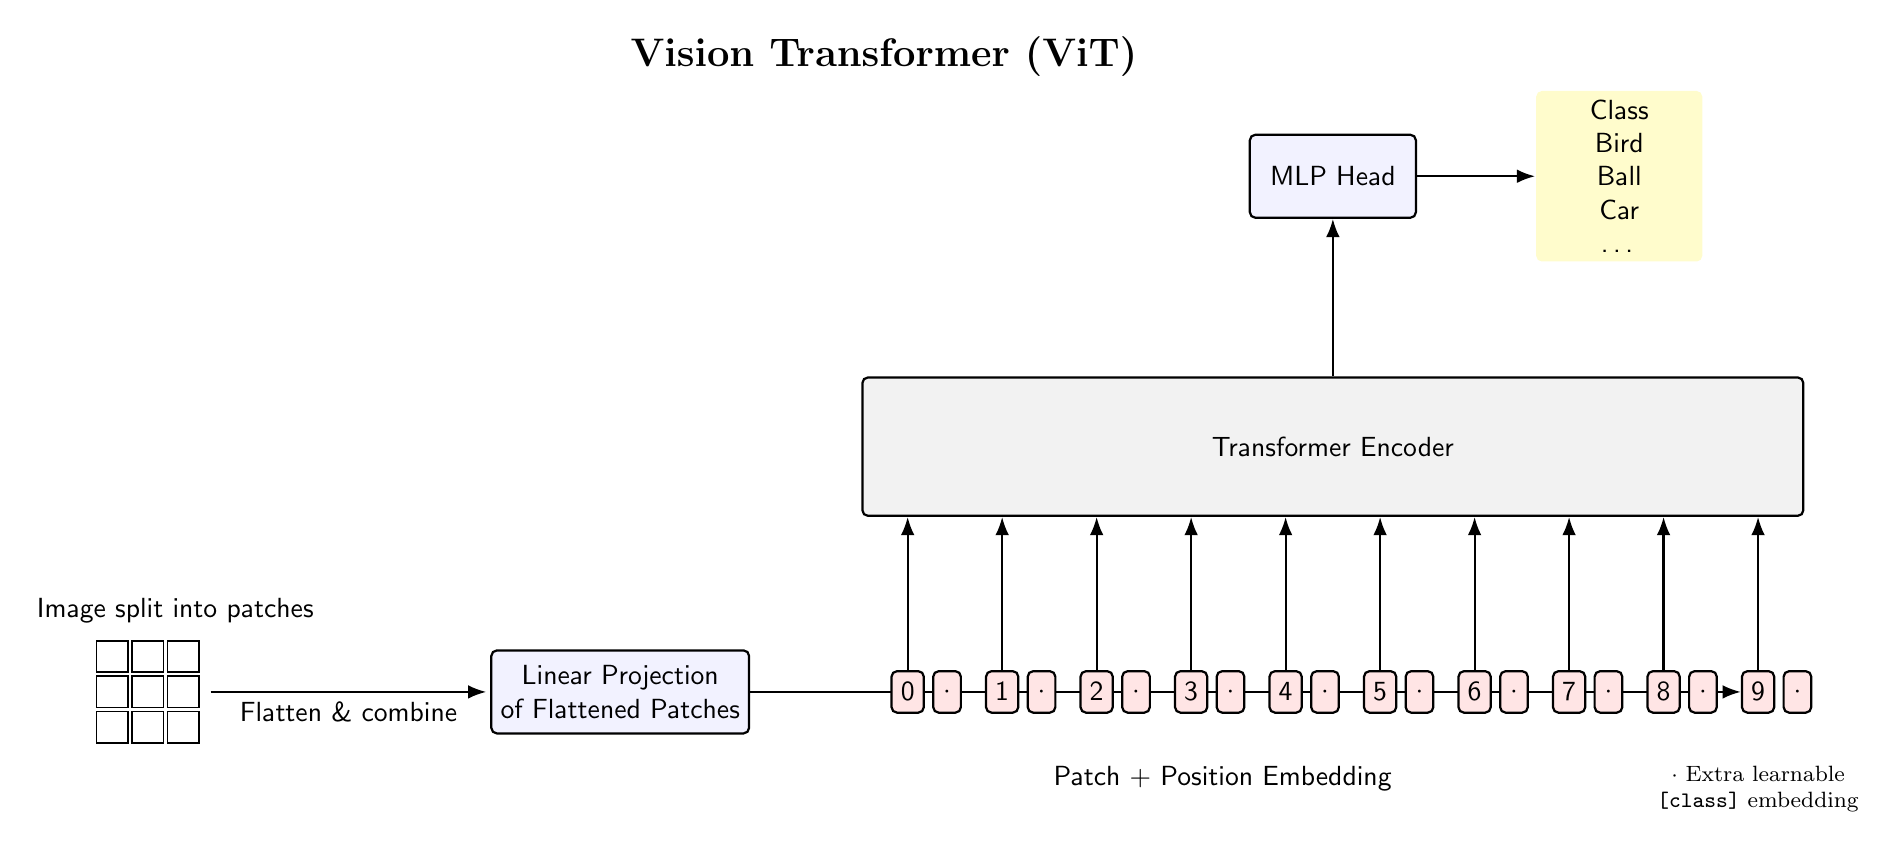
\begin{tikzpicture}[
    font=\sffamily,
    >=LaTeX,
    line width=0.8pt,
    every node/.style={align=center},
    token/.style={draw, rounded corners=2pt, fill=red!10, 
                  minimum width=1.0em, minimum height=1.5em},
    block/.style={draw, thick, rounded corners=2pt, fill=blue!5, 
                  minimum width=6em, minimum height=3em},
    bigblock/.style={draw, thick, rounded corners=2pt, fill=gray!10,
                     minimum width=34em, minimum height=5em}
]

% Title
\node[font=\Large\bfseries, anchor=north] at (6.5,8.2) {Vision Transformer (ViT)};

% 1) Image Patches (3 x 3 grid).
\coordinate (imgorig) at (-3.5,0);
\foreach \j in {0,...,2} {
  \foreach \i in {0,...,2} {
    \draw[line width=0.6pt] 
      ($(imgorig)+(\i*0.45,-\j*0.45)$)
      rectangle ++(0.4,0.4);
  }
}
\node[above] at ($(imgorig)+(1.0,0.5)$) {Image split into patches};

% 2) Arrow into “Linear Projection” block.
\draw[->] ($(imgorig)+(1.45,-0.25)$) -- ++(3.5,0)
      node[midway, below] {Flatten \& combine};

\node[block, anchor=west] (linearproj) at ($(imgorig)+(5.0,-0.25)$)
   {Linear Projection\\of Flattened Patches};

% 3) Tokens after projection + position embedding.
\coordinate[right=2 of linearproj] (tokensleft);
\node[] at ($(tokensleft)+(4.0,-1.1)$) {Patch + Position Embedding};

% Classification token [class].

\node[token] (token9) 
       at ($(tokensleft)+(1.2*9,0)$) {9};



\node[below=1.5em of token9, font=\footnotesize] 
   {$\cdot$ Extra learnable \\ \texttt{[class]} embedding};


% Lines from linear projection to tokens.
\draw[->] (linearproj.east) -- (token9.west|-linearproj.east);
%\foreach \x in {1,...,9} {
 %  \draw[-] (linearproj.east) -- (token\x.west);
%}
\node[token] (token0) at (tokensleft) {0};
\draw[-] (linearproj.east) -- (token0.west);

% Patch tokens labeled “1”…”8”.
\foreach \x in {1,...,8} {
    \node[token] (token\x) 
       at ($(token0)+(1.2*\x,0)$) {\x};
}
\foreach \x in {0,...,9} {
    \node[token] (token\x*) 
       at ($(token0)+ (0.5,0) +(1.2*\x,0)$) {$\cdot$};
}

% 4) Transformer Encoder (shifted further up).
\node[bigblock, anchor=south] (transformer) 
   at ($(token0.south)!0.5!(token9.south) + (0,2.5)$)
   {Transformer Encoder};

% Arrows from each token into the encoder.
\foreach \x in {0,1,...,9} {
    \draw[->] (token\x.north) 
        -- (transformer.south -| token\x.north);
}

% 5) MLP Head above the Transformer.
\node[block, above=2 of transformer.north] (mlphead)
   {MLP Head};
\draw[->] (transformer.north) -- (mlphead.south);

% 6) Class output (shifted further right).
\node[draw=none, fill=yellow!20, rounded corners=2pt,
      minimum width=6em, minimum height=3em,
      right=1.5 of mlphead] (classout)
   {Class\\Bird\\Ball\\Car\\\dots};

\draw[->] (mlphead.east) -- (classout.west);

\end{tikzpicture}
\end{document}
